\documentclass{article}
\usepackage{hyperref}
\usepackage[utf8]{inputenc}
\usepackage[english]{babel}
\usepackage{amsmath}
\usepackage{todonotes}
\usepackage{float}
\usepackage{listings}
\usepackage{gensymb}

\definecolor{mygreen}{RGB}{28,172,0}
\definecolor{mylilas}{RGB}{170,55,241}

\newcommand{\norm}[1]{\left\lVert#1\right\rVert}

\lstset{language=Matlab,%
    %basicstyle=\color{red},
    breaklines=true,%
    morekeywords={matlab2tikz},
    keywordstyle=\color{blue},%
    morekeywords=[2]{1}, keywordstyle=[2]{\color{black}},
    identifierstyle=\color{black},%
    stringstyle=\color{mylilas},
    commentstyle=\color{mygreen},%
    showstringspaces=false,%without this there will be a symbol in the places where there is a space
    numbers=left,%
    numberstyle={\tiny \color{black}},% size of the numbers
    numbersep=9pt, % this defines how far the numbers are from the text
    %emph=[1]{for,end,break},emphstyle=[1]\color{red}, %some words to emphasise
}

\title{Computer Vision I - Sheet 5\\Group 2\\}
\author{ Jonas Otto\\ \href{mailto:jonas@jonasotto.com}{jonas@jonasotto.com} \and Dominik Authaler \\ 
\href{mailto:dominik.authaler@uni-ulm.de}{dominik.authaler@uni-ulm.de}
}

\date{\today}

\begin{document}
\maketitle

\newpage

\section{Gaussian Pyramids}
The source code for this task can be found in the files \texttt{sh05ex01.m} and \texttt{gaussianPyramid.m}. To avoid opening Matlab only for viewing the code, it's included below. 
The results of this exercise are shown in the figures \ref{ex01_with} and \ref{ex01_without}. Comparing the two pyramids, one can see a few differences, but in the overall comparison they look quite similiar.
Nevertheless there should be quite huge differences if one would compare the reconstructed images. Because of the missing gaussian filtering, the reconstructed image of the second pyramid should show a low of distortions. 
\begin{figure}[H]
  \begin{center}
    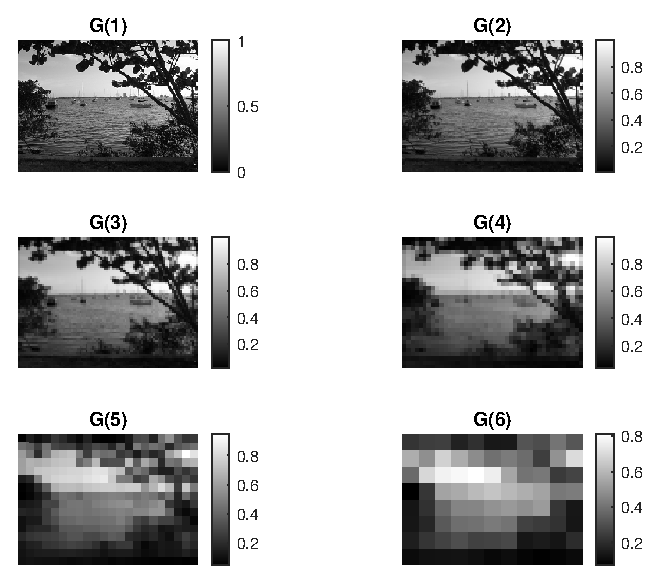
\includegraphics[width=\textwidth]{./images/ex01_with.eps}
    \caption{Gaussian pyramid with Gaussian filtering}
    \label{ex01_with}
  \end{center}
\end{figure}

\begin{figure}[H]
  \begin{center}
    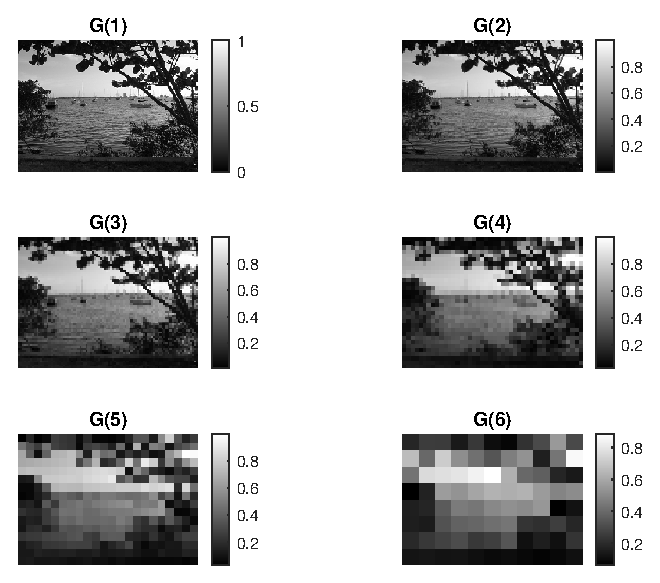
\includegraphics[width=\textwidth]{./images/ex01_without.eps}
    \caption{Gaussian pyramid without Gaussian filtering}
    \label{ex01_without}
  \end{center}
\end{figure}

\hspace{20mm}
\lstinputlisting{./matlab/sh05ex01.m}

\hspace{20mm}
\lstinputlisting{./matlab/gaussianPyramid.m}



\clearpage
\section{Laplacian Pyramids}
The source code for this task can be found in the files \texttt{sh05ex02.m} and \texttt{reconstruct.m} or below. Figure \ref{ex02_pyr} shows the generated Laplacian pyramid, the corresponding reconstructed image is shown in figure \ref{ex02_rec}. The figures \ref{ex02_pyr_comp} and \ref{ex02_rec_comp} show the same Laplacian pyramid where compression was applied. Obviously the compression wasn't lossless, as the image no has quite huge artifacts in it. 
Figure \ref{ex02_error} shows the resulting error of the compression for different threshold levels. As one would expect, the error raises with the threshold value, because more values are treated as zero. 


\begin{figure}[H]
  \begin{center}
    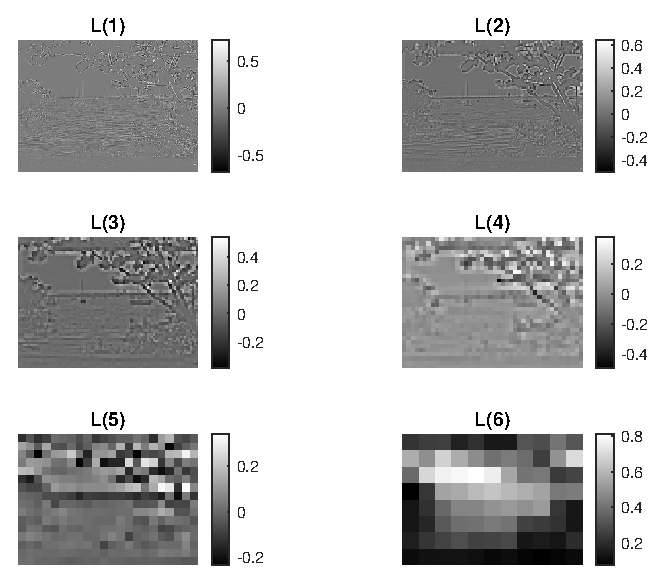
\includegraphics[width=\textwidth]{./images/ex02_pyramid.eps}
    \caption{Laplacian pyramid}
    \label{ex02_pyr}
  \end{center}
\end{figure}

\begin{figure}[H]
  \begin{center}
    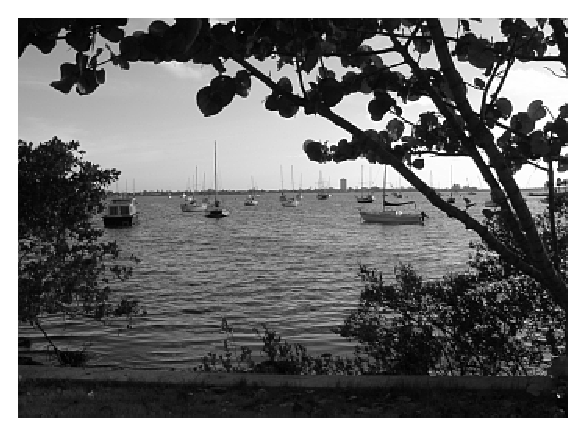
\includegraphics[width=\textwidth]{./images/ex02_reconstructed.eps}
    \caption{Reconstructed image}
    \label{ex02_rec}
  \end{center}
\end{figure}

\begin{figure}[H]
  \begin{center}
    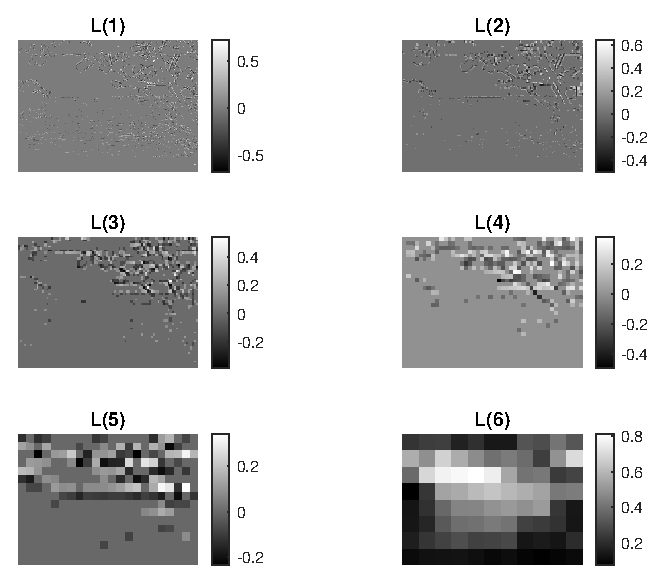
\includegraphics[width=\textwidth]{./images/ex02_pyr_compress.eps}
    \caption{Laplacian pyramid with applied compression}
    \label{ex02_pyr_comp}
  \end{center}
\end{figure}

\begin{figure}[H]
  \begin{center}
    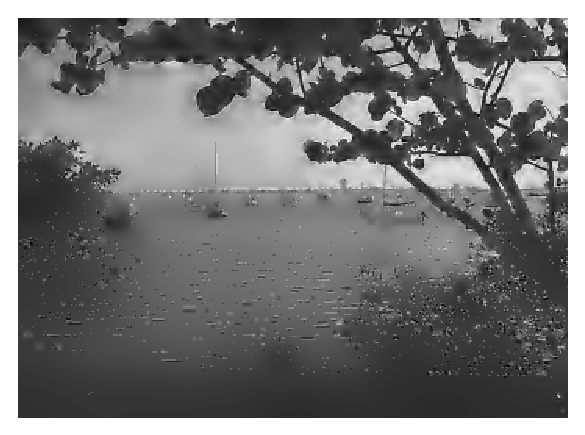
\includegraphics[width=\textwidth]{./images/ex02_rec_compress.eps}
    \caption{Reconstructed image from the compressed pyramid}
    \label{ex02_rec_comp}
  \end{center}
\end{figure}

\begin{figure}[H]
  \begin{center}
    \includegraphics[width=\textwidth]{./images/ex02_error.eps}
    \caption{Error for different threshold values}
    \label{ex02_error}
  \end{center}
\end{figure}

\hspace{20mm}
\lstinputlisting{./matlab/sh05ex02.m}

\hspace{20mm}
\lstinputlisting{./matlab/reconstruct.m}

\clearpage
\section{Gabor wavelets}
The source code for this task can be found in the file \texttt{sh05ex03.m} or below. The Matlab script for the \texttt{getGabor} function was given in the exercise. 
Figure \ref{ex03} shows the results of the energy calculations. On can easily stand, that the main orientations of the texture in the image are vertical and horizontal, because this orientations showed the biggest results.
\begin{figure}[H]
  \begin{center}
    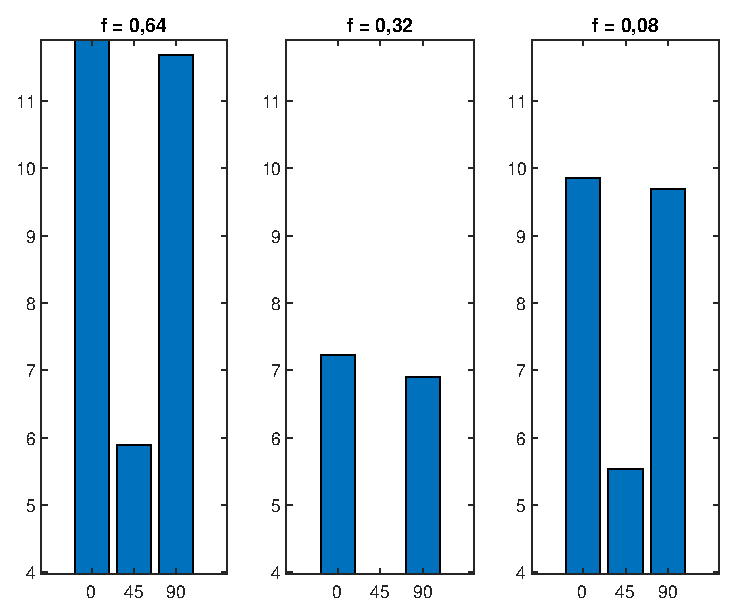
\includegraphics[width=\textwidth]{./images/ex03.eps}
    \caption{Filter energy of the different Gabor wavelets}
    \label{ex03}
  \end{center}
\end{figure}

\hspace{20mm}
\lstinputlisting{./matlab/sh05ex03.m}

\end{document}

